%====================================================================
\subsection*{Directed networks} 
%====================================================================
\frame{\frametitle{Conditional independance}

  \paragraph{Definition.} $X$ is independent of $Y$ conditional on $Z$ ($X \independent Y \mid Z$) iff
  $$
  p(x, y \mid z) = p(x \mid z) p(y \mid z)
  \qquad \Leftrightarrow \qquad 
  p(x \mid z, y) = p(x \mid z) 
  $$

  \bigskip \bigskip \pause
  \paragraph{Example.} $A \independent C \mid B$ in the 3 DAGs:
  $$
    \begin{tikzpicture}
  \node[observed] (x) at (0*\edgeunit, 0*\edgeunit) {$X$};
  \node[observed] (y) at (1*\edgeunit, 0*\edgeunit) {$Y$};
  \node[observed] (z) at (2*\edgeunit, 0*\edgeunit) {$Z$};
  
  \draw[arrow] (x) to (y);  \draw[arrow] (y) to (z);
  \end{tikzpicture}
 \qquad
    \begin{tikzpicture}
  \node[observed] (x) at (0*\edgeunit, 0*\edgeunit) {$X$};
  \node[observed] (y) at (1*\edgeunit, 0*\edgeunit) {$Y$};
  \node[observed] (z) at (2*\edgeunit, 0*\edgeunit) {$Z$};
  
  \draw[arrow] (z) to (y);  \draw[arrow] (y) to (x);
  \end{tikzpicture}
 \qquad
    \begin{tikzpicture}
  \node[observed] (x) at (0*\edgeunit, 0*\edgeunit) {$X$};
  \node[observed] (y) at (1*\edgeunit, 0*\edgeunit) {$Y$};
  \node[observed] (z) at (2*\edgeunit, 0*\edgeunit) {$Z$};
  
  \draw[arrow] (y) to (z);  \draw[arrow] (y) to (x);
  \end{tikzpicture}

  $$
  Indeed, for first one,
  $$
  p(x, z \mid y)
  = \frac{p(x, y, z)}{p(y)}
  = \frac{p(x) p(y \mid x) p(z \mid y)}{p(y)}
  = p(x \mid y) p(z \mid y)
  $$
  because $p(x) p(y \mid x) = p(y) p(x \mid y)$.
}

%====================================================================
\frame{\frametitle{V-structure}

%   \paragraph{Counter-example.} 
  In the V-structured (or 'head to head') DAG:
  $$
    \begin{tikzpicture}
  \node[observed] (x) at (0*\edgeunit, 0*\edgeunit) {$X$};
  \node[observed] (y) at (1*\edgeunit, 0*\edgeunit) {$Y$};
  \node[observed] (z) at (2*\edgeunit, 0*\edgeunit) {$Z$};
  
  \draw[arrow] (x) to (y);  \draw[arrow] (z) to (y);
  \end{tikzpicture}

  $$
  $X$ and $Z$ are \emphase{conditionally dependent} ($X \not\independent Y \mid Z$):
  \begin{align*}
  p(x, y, z) & = p(x) p(z) p(y \mid x, z) \\ ~\\
  \Rightarrow \quad
  p(x, z \mid y) & = \frac{p(x, y, z)}{p(y)}   = \frac{p(x) p(z) p(y \mid x, z)}{p(y)}  
  \end{align*}
  
  \bigskip \bigskip \pause
  \paragraph{Remark.} 
  $X$ and $Z$ are \emphase{marginally independent}:
  $$
   p(x, z)
  = \sum_y p(x) p(z) p(y \mid x, z)
  = p(x) p(z) \underset{= 1}{\underbrace{\sum_y p(y \mid x, z)}}
  $$
}


%====================================================================
\frame{\frametitle{From directed to undirected graphical models}

  \paragraph{Resolve {\sl immoralities}.} Graph {\sl moralization} (parents must be married):
  $$
  \begin{array}{ccccc}
     \begin{tikzpicture} 
    \node[observed] (a) at (0*\edgeunit, 1*\edgeunit) {$A$};
  \node[observed] (b) at (1*\edgeunit, 1*\edgeunit) {$B$};
  \node[observed] (c) at (.5*\edgeunit, 0*\edgeunit) {$C$};
  

  
  \draw[arrow] (a) to (c);  \draw[arrow] (b) to (c);
  \end{tikzpicture}
  

   & \qquad & 
     \begin{tikzpicture} 
    \node[observed] (a) at (0*\edgeunit, 1*\edgeunit) {$A$};
  \node[observed] (b) at (1*\edgeunit, 1*\edgeunit) {$B$};
  \node[observed] (c) at (.5*\edgeunit, 0*\edgeunit) {$C$};
  

  
  \draw[arrow] (a) to (c);  \draw[arrow] (b) to (c);
  \draw[dashededge] (a) to (b);
  \end{tikzpicture}
  

   & \qquad & 
     \begin{tikzpicture} 
    \node[observed] (a) at (0*\edgeunit, 1*\edgeunit) {$A$};
  \node[observed] (b) at (1*\edgeunit, 1*\edgeunit) {$B$};
  \node[observed] (c) at (.5*\edgeunit, 0*\edgeunit) {$C$};
  

  
  \draw[edge] (a) to (c);  \draw[edge] (b) to (c);
  \draw[edge] (a) to (b);
  \end{tikzpicture}
  

  \end{array}
  $$
  
  \pause
  \paragraph{Example.}
  $$
  \begin{array}{ccccc}
     \begin{tikzpicture}
    \node[observed] (a) at (.5*\edgeunit, 2.75*\edgeunit) {$A$};
  \node[observed] (b) at (0*\edgeunit, 2*\edgeunit) {$B$};
  \node[observed] (c) at (1*\edgeunit, 2*\edgeunit) {$C$};
  \node[observed] (d) at (0.5*\edgeunit, 1*\edgeunit) {$D$};
  \node[observed] (e) at (0*\edgeunit, 0*\edgeunit) {$E$};
  \node[observed] (f) at (1*\edgeunit, 0*\edgeunit) {$F$};

  
  \draw[arrow] (a) to (b);  \draw[arrow] (a) to (c);
  \draw[arrow] (b) to (d);  \draw[arrowbendleft] (b) to (f);
  \draw[arrow] (c) to (d);  \draw[arrow] (d) to (e);
  \draw[arrow] (d) to (f);  
  \end{tikzpicture}

   & \qquad & 
     \begin{tikzpicture}
    \node[observed] (a) at (.5*\edgeunit, 2.75*\edgeunit) {$A$};
  \node[observed] (b) at (0*\edgeunit, 2*\edgeunit) {$B$};
  \node[observed] (c) at (1*\edgeunit, 2*\edgeunit) {$C$};
  \node[observed] (d) at (0.5*\edgeunit, 1*\edgeunit) {$D$};
  \node[observed] (e) at (0*\edgeunit, 0*\edgeunit) {$E$};
  \node[observed] (f) at (1*\edgeunit, 0*\edgeunit) {$F$};

  
  \draw[arrow] (a) to (b);  \draw[arrow] (a) to (c);
  \draw[dashededge] (b) to (c);  
  \draw[arrow] (b) to (d);  \draw[arrowbendleft] (b) to (f);
  \draw[arrow] (c) to (d);  \draw[arrow] (d) to (e);
  \draw[arrow] (d) to (f);  
  \end{tikzpicture}

   & \qquad & 
     \begin{tikzpicture}
    \node[observed] (a) at (.5*\edgeunit, 2.75*\edgeunit) {$A$};
  \node[observed] (b) at (0*\edgeunit, 2*\edgeunit) {$B$};
  \node[observed] (c) at (1*\edgeunit, 2*\edgeunit) {$C$};
  \node[observed] (d) at (0.5*\edgeunit, 1*\edgeunit) {$D$};
  \node[observed] (e) at (0*\edgeunit, 0*\edgeunit) {$E$};
  \node[observed] (f) at (1*\edgeunit, 0*\edgeunit) {$F$};

  
  \draw[edge] (a) to (b);  \draw[edge] (a) to (c);
  \draw[edge] (b) to (c);  
  \draw[edge] (b) to (d);  \draw[edgebendleft] (b) to (f);
  \draw[edge] (c) to (d);  \draw[edge] (d) to (e);
  \draw[edge] (d) to (f);  
  \end{tikzpicture}

  \end{array}
  $$
}

%====================================================================
\subsection*{Causality}
%====================================================================
\frame{\frametitle{Causality \refer{Pea09}}

  \begin{tabular}{c|c|c}
    'Truth' & Equivalent & 'Causality' \\  
    & {based on observational data} \\  
    & & \\\hline & & \\
    \includegraphics[trim={0 15 180 0}, height=.22\textheight, clip]{\figeco/Pea09-Fig2-3}
    &
    \includegraphics[trim={0 15 0 0}, height=.21\textheight, clip]{\figeco/Pea09-Fig2-4}
    &
    \includegraphics[trim={180 15 0 0}, height=.22\textheight, clip]{\figeco/Pea09-Fig2-3}
  \end{tabular}

  \bigskip \bigskip 
  $$
  \{a \leftrightarrow b\} \qquad = \qquad \{a \leftarrow u \rightarrow b, 
  \quad \text{$u$ unobserved}\}
  $$  
}

%====================================================================
\subsection*{Dynamic networks}
% %==================================================================
% \frame{\frametitle{Lotka-Voltera interpretation}
% 
%   \begin{itemize}
%   \item Review \& methods: \refer{FLG15}
%   \item Fundamental limitations: \refer{AML17} ('all state variables are measured without any measurement noise') + \refer{Ver12}
%   \item Actually doable? Steady-state approach: \refer{XAF17}
%   \item Lotka-Volterra (simul): \refer{BeW14}
%   \item Lotka-Volterra micro: \refer{SBT13}
%   \item Pseudo Lotka-Volterra: \refer{AHL12}, \refer{FaR12}
%   \item Likelihood-free approach (Lotka-Volterra as an example): \refer{TRB17}
%   \end{itemize}
% }
% 
%====================================================================
\subsection*{Latent GGM}
%==================================================================
\frame{\frametitle{Effect of covariates}

  \paragraph{Fish species in the Fatala river \refer{Bar95}.} $n = 95$ observations, $p = 33$ fish species, $x_i =$ date and site of the observations

  \bigskip \bigskip 
  \paragraph{Inferred networks.} 
  $$
  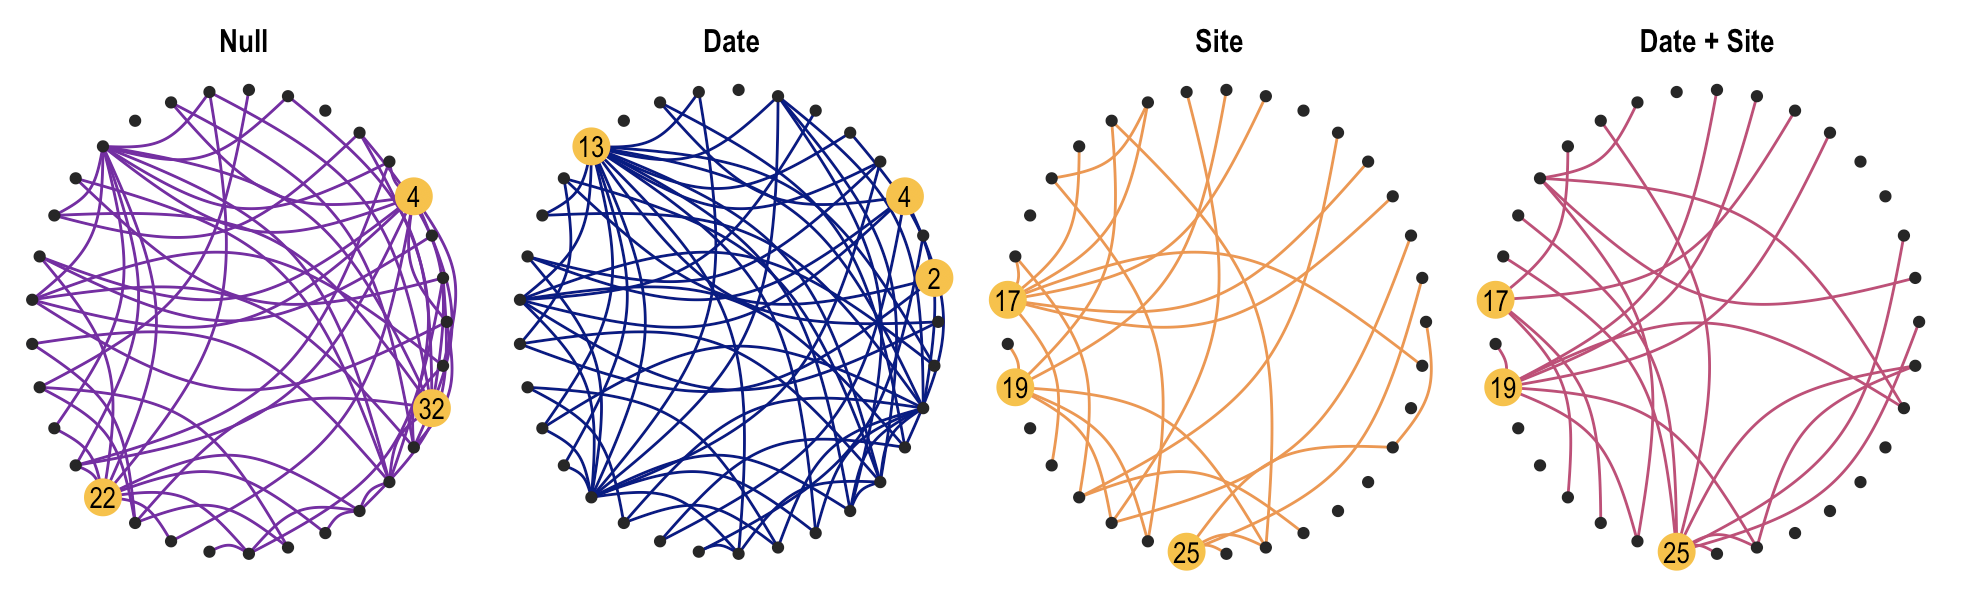
\includegraphics[width=.9\textwidth]{\fignet/MRA19-Fig8} 
  $$
  \ra Even 'key-species' change according to which covariates are taken into account.
}
